%for slideshow
%\documentclass[ignorenonframetext]{beamer} %add option 'draft' for quicker compilation
%\usepackage{beamerthemesplit}
%\newcommand{\slides}{1}
%\includeonlyframes{current} %this only compiles frames with [label=current]
 
%for handouts
\documentclass[a4paper,12pt]{article}
\usepackage{beamerarticle}
\newcommand{\slides}{0}

\mode<article>
{
	\usepackage[colorlinks,
	pdfauthor="Len Thomas",
	pdftitle="MT4113 Lecture notes"]{hyperref}
    \usepackage[a4paper,margin=1cm,footskip=.5cm]{geometry}
}
\mode<presentation>
{
%    \usetheme{Singapore}
  \pgfdeclareimage[height=1cm]{StA-logo}{logo}
  \logo{\pgfuseimage{StA-logo}}
    \usetheme{EastLansing}
%    \usetheme{JuanLesPins}
    	\usecolortheme{sidebartab}
	\setbeamertemplate{navigation symbols}{\insertsectionnavigationsymbol}
}

\usepackage[english]{babel}
\usepackage[latin1]{inputenc}
\usepackage[sfdefault]{cabin}
\usepackage[T1]{fontenc}
\usepackage{epsf,graphics,graphicx,fancyhdr,color,amsmath,url,enumerate,alltt}
\usepackage{ifthen}

\newcommand{\bc}{\begin{center}}
\newcommand{\ec}{\end{center}}
\newcommand{\bn}{\begin{enumerate}}
\newcommand{\en}{\end{enumerate}}
\newcommand{\bi}{\begin{itemize}}
\newcommand{\ei}{\end{itemize}}
\newcommand{\be}{\begin{eqnarray}}
\newcommand{\ee}{\end{eqnarray}}
\newcommand{\bes}{\begin{eqnarray*}}
\newcommand{\ees}{\end{eqnarray*}}

\title[MT4113]{MT 4113: Computing in Statistics}

\subtitle{Computer intensive statistics\\Lecture 7: The Bootstrap}

\author[Lecture 7]{Len Thomas}

%\institute{School of Mathematics and Statistics, University of St Andrews}

\date[15/10/2018] {15 Oct 2018}

\mode<presentation> {
    \AtBeginSection[]
    {
    \begin{frame}<beamer>
        \frametitle{Outline}
        \tableofcontents[currentsection,currentsubsection]
    \end{frame}
    }
    \AtBeginSubsection[]
    {
    \begin{frame}<beamer>
        \frametitle{Outline}
        \tableofcontents[currentsection,currentsubsection]
    \end{frame}
    }
}
\begin{document}

\begin{frame}
  \titlepage
\end{frame}

\mode<article>{
\maketitle
}

\section{Introduction and recap}


\begin{frame}[fragile]
\frametitle{Repeated sampling: the basis for inference}
In classical (``frequentist'') statistics, we rely on the concept of repeated sampling to make inferences about the quantity of interest -- e.g., the population mean.
\bi
\item <2-> Hypothesis testing: if I could repeat the experiment many times and H0 was true, what proportion of sample means would be as extreme or more extreme than my value?
\item <3-> Confidence intervals: if I could repeat the experiment many times, what interval would contain the population mean a specified proportion of times?
\ei
\end{frame}

\begin{frame}[fragile]
\mode<presentation>{\frametitle{Repeated sampling: the basis for inference}}
In both cases, the ``ideal'' would be to have multiple replicate datasets.
\bi
\item <2->Hypothesis testing: same data generating process as our data, but where H0 is true.  Can then see how extreme our sample mean is.
\item <3->Confidence intervals: 
   \bi 
	 \item <4->Invert the test statistic: same data generating process as our data, but over a range of hypothesized means.  Can see which hypothesized means are plausible -- those where our sample mean is not extreme.
	 \item <5->Alternative: exact same data generating process as our data -- i.e. with the same true population mean.  Can generate a distribution of plausible sample means and assume they represent the distribution of plausible population means.
	 \ei
\ei
But, we only have the one dataset to use...
\end{frame}

\begin{frame}[fragile]
\frametitle{Computer-intensive inference}
Use properties of the dataset we have to help us \emph{simulate} repeated datasets.
\bi
\item <2->Hypothesis testing -- Monte Carlo tests -- simulate data with H0 true.
\item <3->Confidence intevals:
\bi
\item <4->Invert test statistic -- simulate data with a range of values of H0.
\item <5->Simulate data as close as possible to the data generating process -- ``resamples''.  This is the bootstrap.
\ei
\ei

Note, simulations can be:
\bi
\item <6->Nonparametric: sample from the data to create new datasets.
\item <7->Parametric: simulate from a distribution based on the data to create new datasets.
\ei
\end{frame}


\section{Nonparametric bootstrap}

\subsection{How to generate resamples}

\begin{frame}
    \frametitle{Empirical distribution function (EDF)}
    \bc
        	\mode<presentation>
        	  {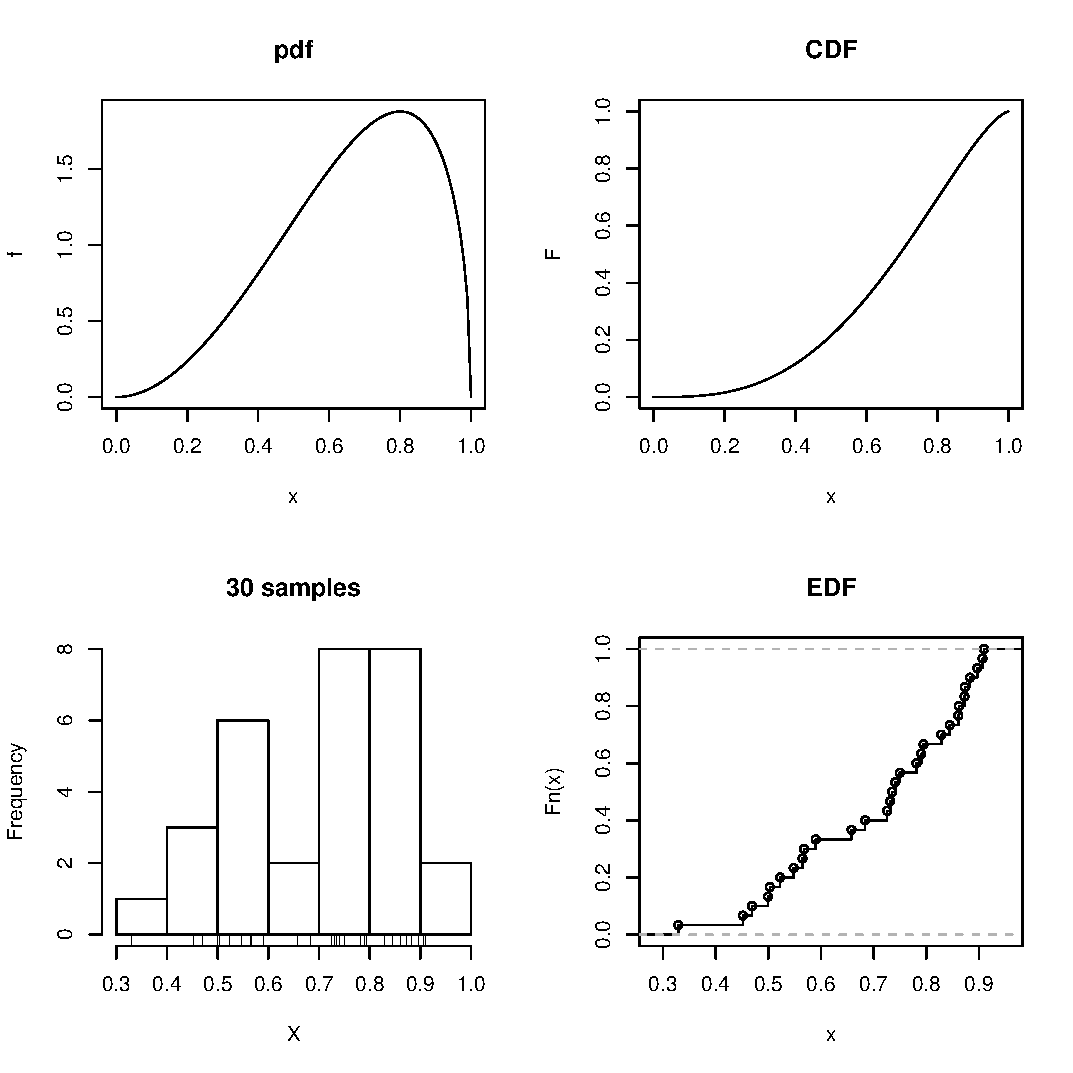
\includegraphics[height=2.7in]{edf}}
        	 \mode<article> {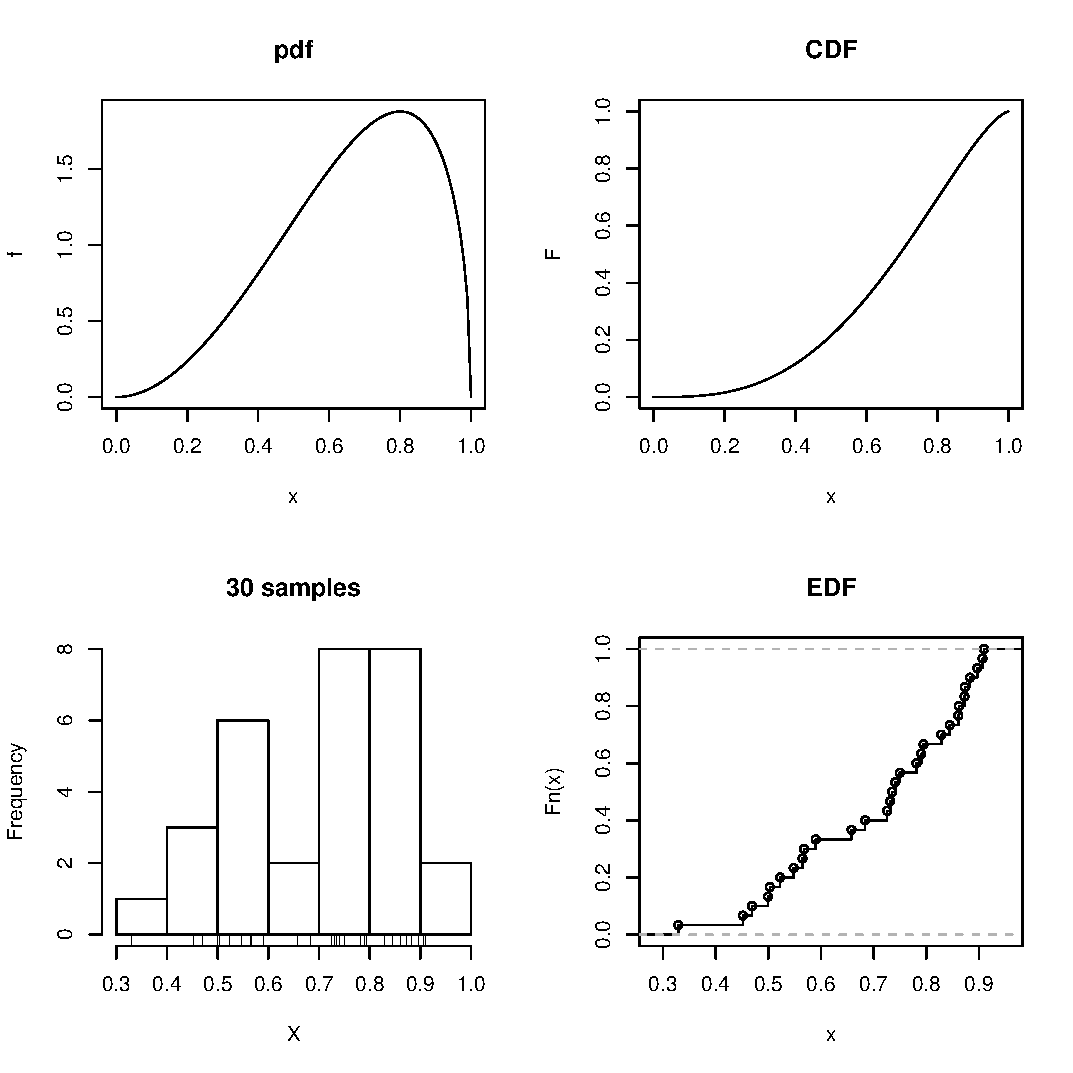
\includegraphics[height=2.0in]{edf}}
    \ec
\end{frame}

\begin{frame}[fragile]
    \frametitle{Nonparametric bootstrap and the EDF}
    \bi
        \item <1-> Nonparametric bootstrap:
        \bi
            \item generate resamples by simulating from the EDF
            \item produces resamples that have the same properties as the data (c.f. previous methods where they had the same properties if $H0$ was true)
						\item best approximation we have to sampling again from the original data generating process
        \ei
        \item <2->How to sample from the EDF?
        \bi
            \item Resample with replacement from the data
        \ei
    \ei
\end{frame}

\begin{frame}
    \frametitle{Pine martin example}
\bc{\Tiny
\begin{tabular}{||r|c|c|c|c|c|c|c|c|c|c|c|c||}
\hline
\hline
Original & 0.13& -0.01& -0.01&  0.42& -0.02&  0.01&  0.09&  0.03&  0.04&  0.06&  0.12&  0.03\\
\hline
\hline
Resamples\\
 1 &0.01& -0.01& -0.02&  0.04& -0.01&  0.13&  0.03& -0.01&  0.03&  0.06&  0.13&  0.09\\
2 &0.09  &0.09& -0.02& -0.01&  0.09&  0.42 & 0.03 &-0.01&  0.04& -0.01&  0.03&  0.03\\
3 &  0.42&  0.03& -0.01&  0.09&  0.06&  0.06&  0.06& -0.02& -0.01&  0.09&  0.4&  0.09\\
$\vdots$\\
$b$ & 0.03  &0.04 & 0.42& 0.09 &-0.01 &-0.01 & 0.03 & 0.04 & 0.13 & 0.03 & 0.09& -0.01\\
\hline
\hline
\end{tabular}
}\ec
\vspace{0.1in}
    \bi
        \item Notes:
        \bi
            \item number of times each data point occurs in each resample is a random variable
            \item in $b$ bootstrap resamples, we expect each data point to appear on average $b$ times
            \item can ensure they occur exactly $b$ times with using a \textit{balanced bootstrap} (but usually not worth the extra effort)
        \ei
    \ei

\end{frame}

\subsection{Bootstrap confidence interval}

\begin{frame}
    \frametitle{Bootstrap confidence intervals}
    \bi
        \item There are many ways to generate a confidence interval via bootstrap resampling\footnote{see, e.g., Carpinter, J. and J. Bithell. (2000) Bootstrap confidence intervals: when, which, what? A practical guide for medical statisticians. Statistics in Medicine 19: 1141-1164.}
        \item Today, we will cover the simplest -- the ``percentile method''
		\ei
\end{frame}


\begin{frame}
    \frametitle{Percentile method}
    \bi
        \item A useful approximate method for producing CIs
				\item Besides being relatively simple to understand and implement, it performs well in practice under most commonly-encountered situations
        \item Very widely used in applied statistics
    \ei
\end{frame}

\begin{frame}[fragile]
    \frametitle{Percentile method -- Rationale}
    \bi
        \item <1->Our resamples come from the same distribution as the original data
        \item <2->So can use the resamples to obtain the distribution of the quantity of interest -- e.g., $\mu$
        \item <3->Example: mean of pine martin data:
    \ei
    \visible<3> {\bc
        \mode<presentation>
          {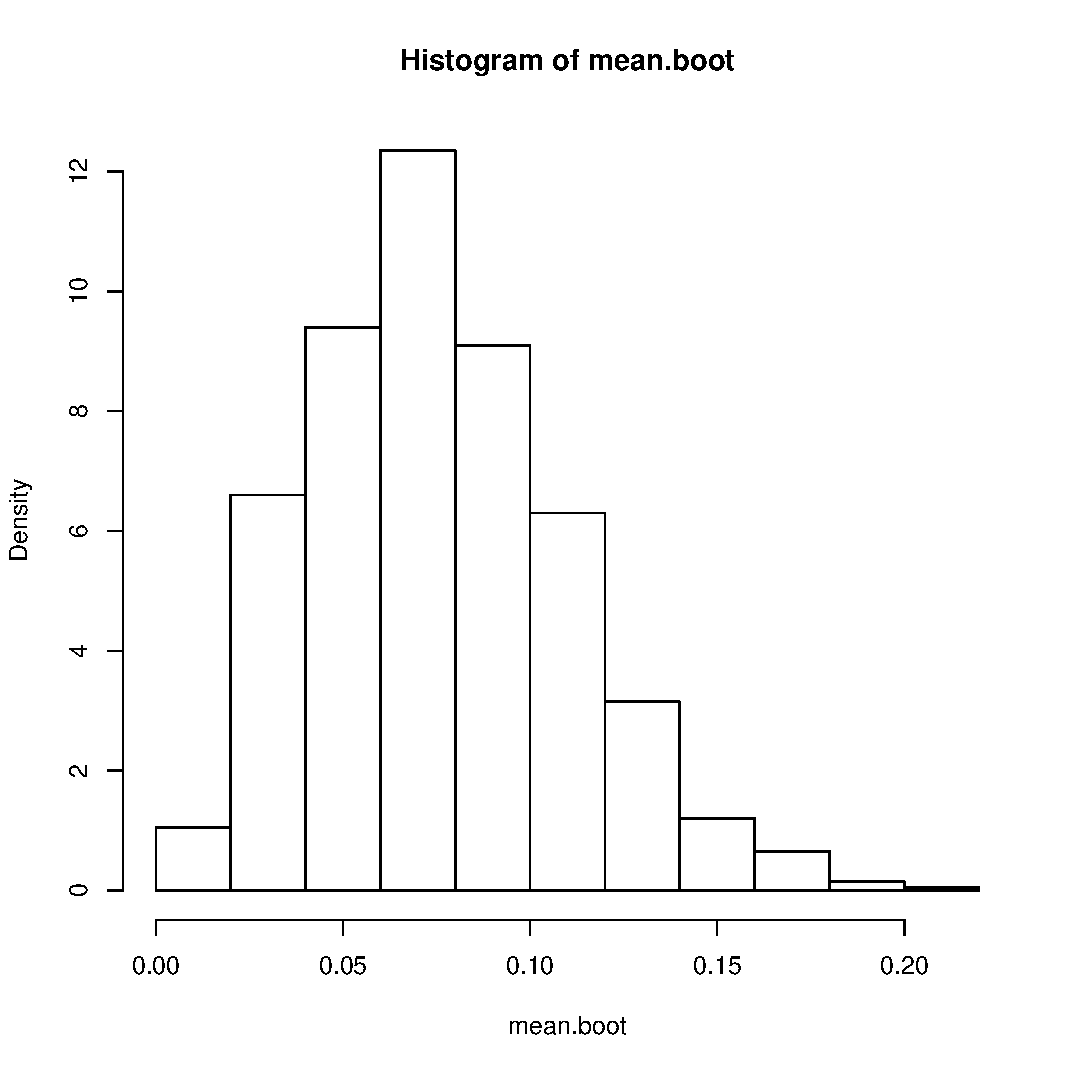
\includegraphics[height=1.7in]{HistMeanBoot}}
        \mode<article>  {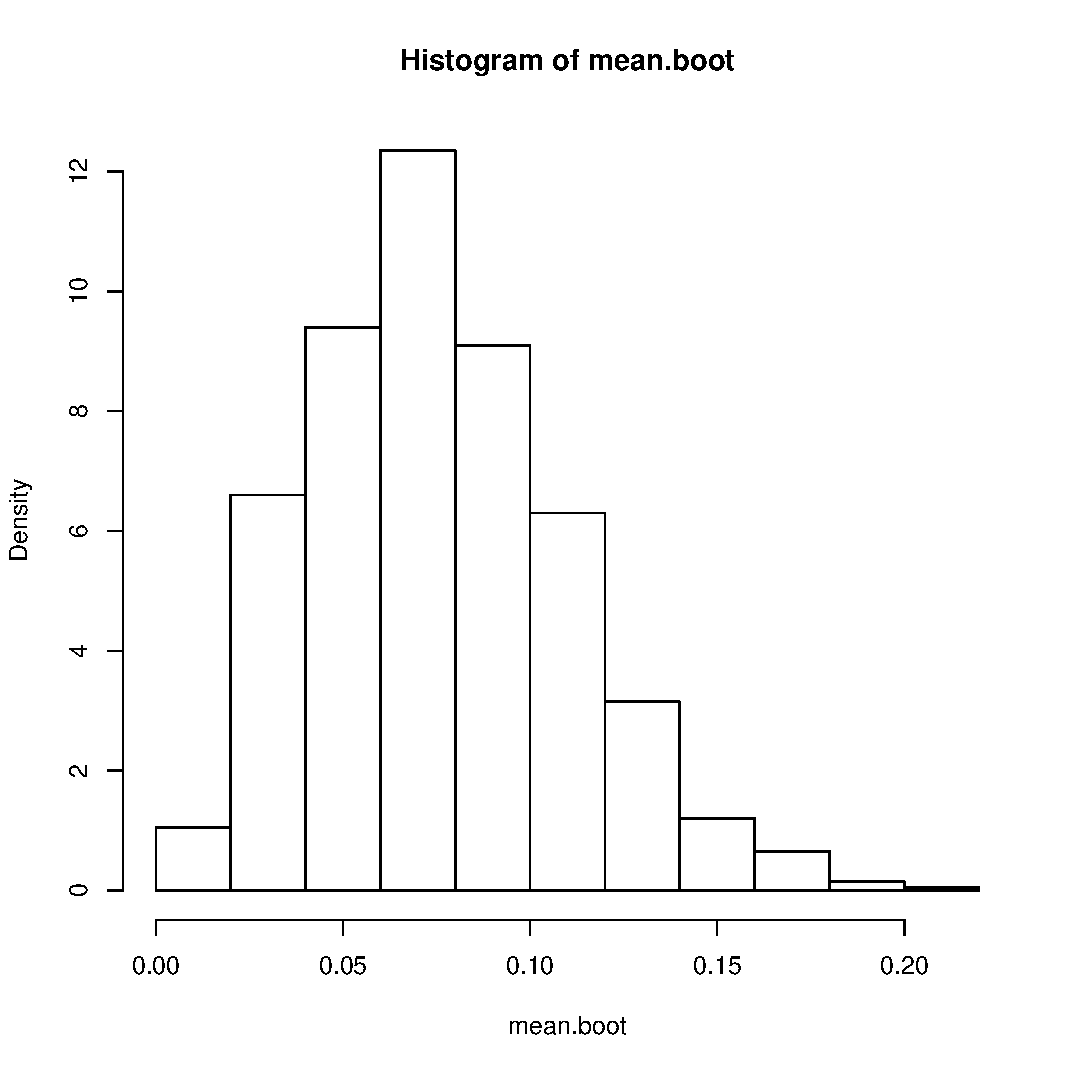
\includegraphics[height=1.5in]{HistMeanBoot}}
    \ec}
\end{frame}

\begin{frame}[fragile]
    \frametitle{Percentile method (contd.)}
    \bi
        \item <1->CI is an interval that contains the true value of $\mu$ $100(1-\alpha)\%$ of the time
        \item <2->Turns out (under some conditions), the following procedure gives an interval with this property:
				\bi
				  \item <2-> Order the $\mu$\\
				  \item <2-> Lower limit is the $\alpha/2(b+1)$\%th value\\
				  \item <2-> Upper limit is the $(1-\alpha/2)(b+1)$\%th value
%If you imagine that we were resampling from the original data generating process, then the distribution of bootstrap means is
% the distribution we'd get from the data generating process, so choosing these quantils means that 95% of the values we get
% will lie within this interval.
%But how is that the same as giving a statement about the true population mean lying in that interval?
        \ei
        \item <3->E.g. For 999 resamples 95\% limits given by the 25th smallest and 25th largest
    \ei
    \visible<4> {\bc
        \mode<presentation>
          {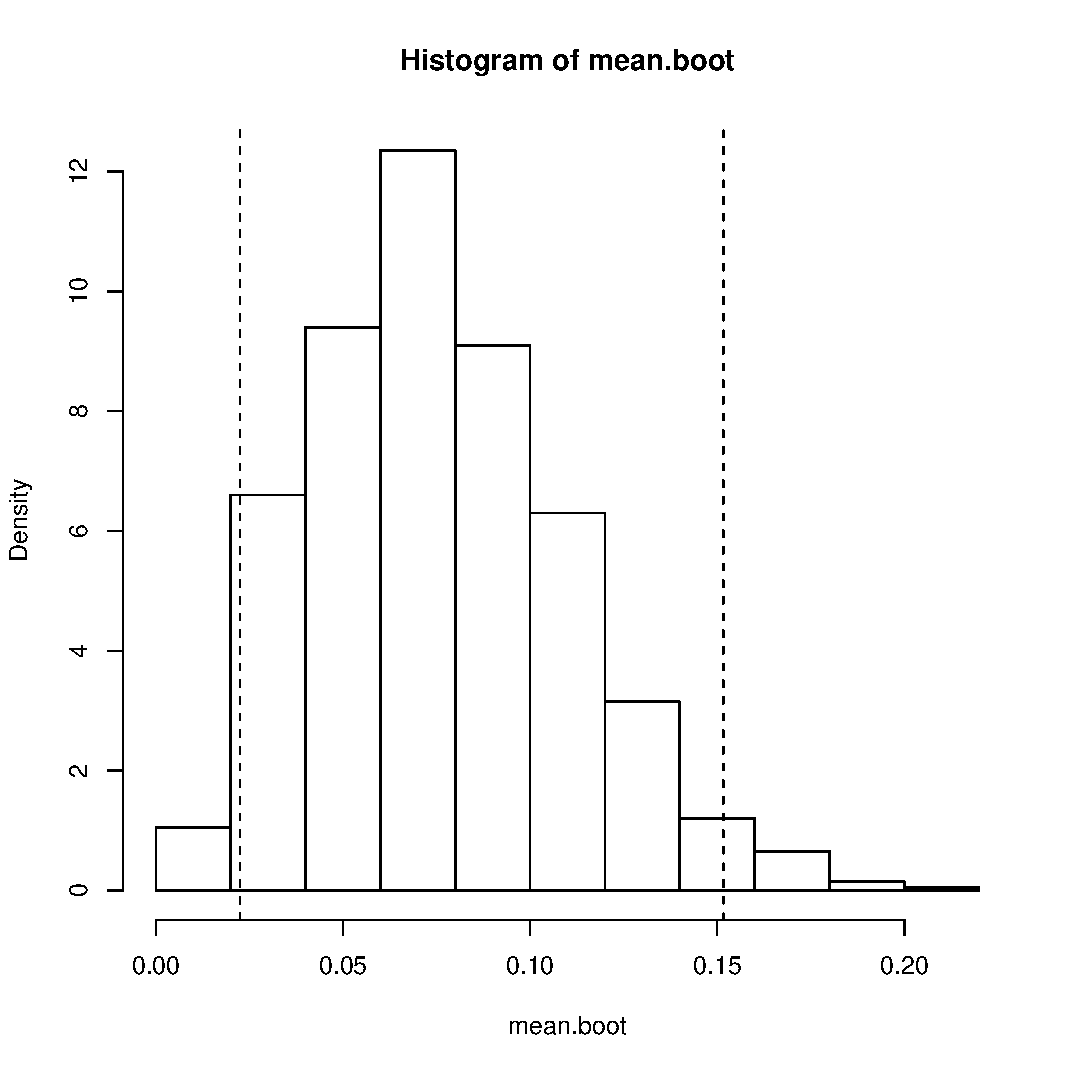
\includegraphics[height=1.4in]{HistMeanBootCI}}
        \mode<article>  {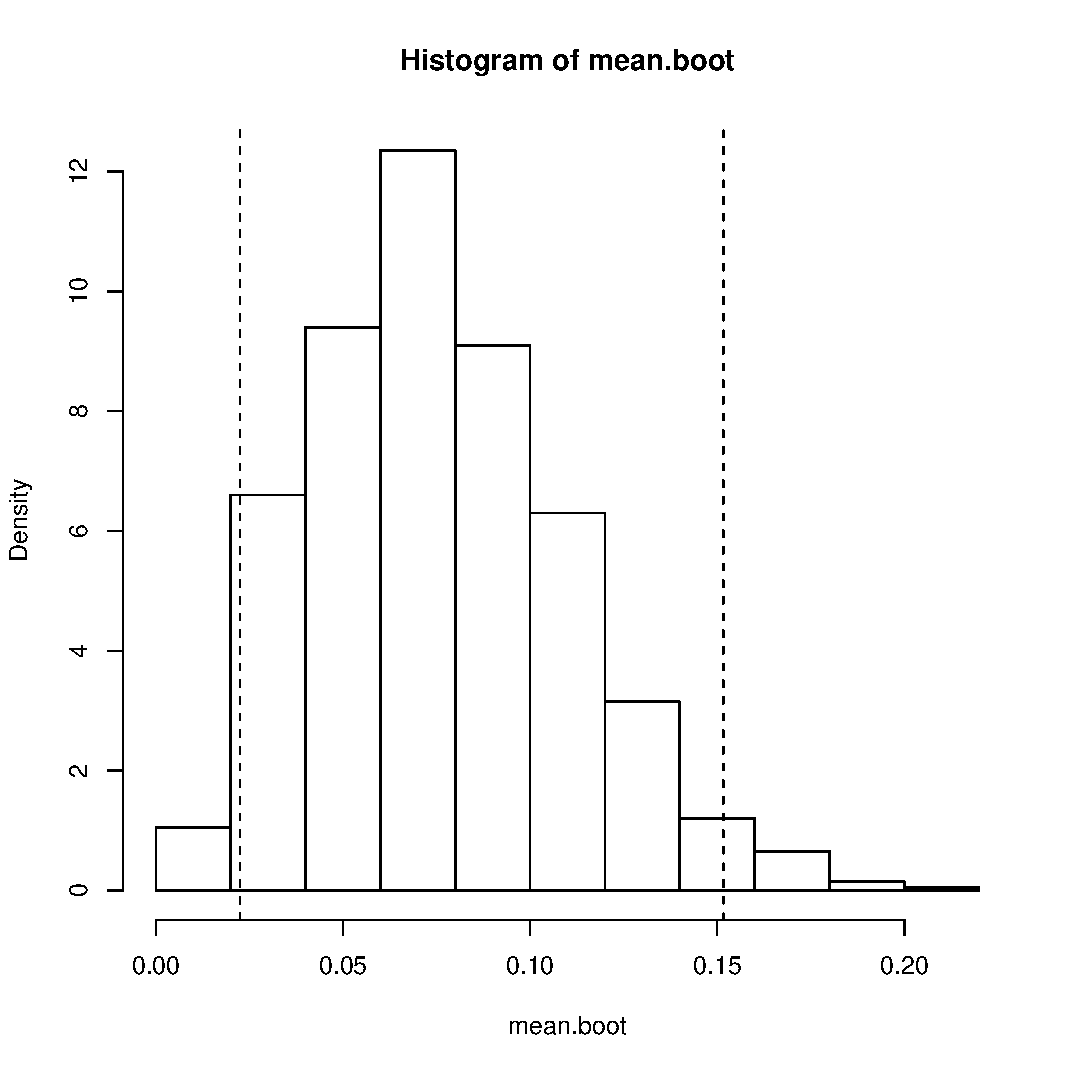
\includegraphics[height=1.5in]{HistMeanBootCI}}
    \ec}
\end{frame}

\begin{frame}[fragile]
    \frametitle{Example}
    \bi
        \item <1->This method is easy to apply and very general, so widely used
        \item <2->Example: distance sampling surveys of wildlife populations \\ (other examples in the reading)
		\mode<presentation>{
    \visible<2> {\bc
						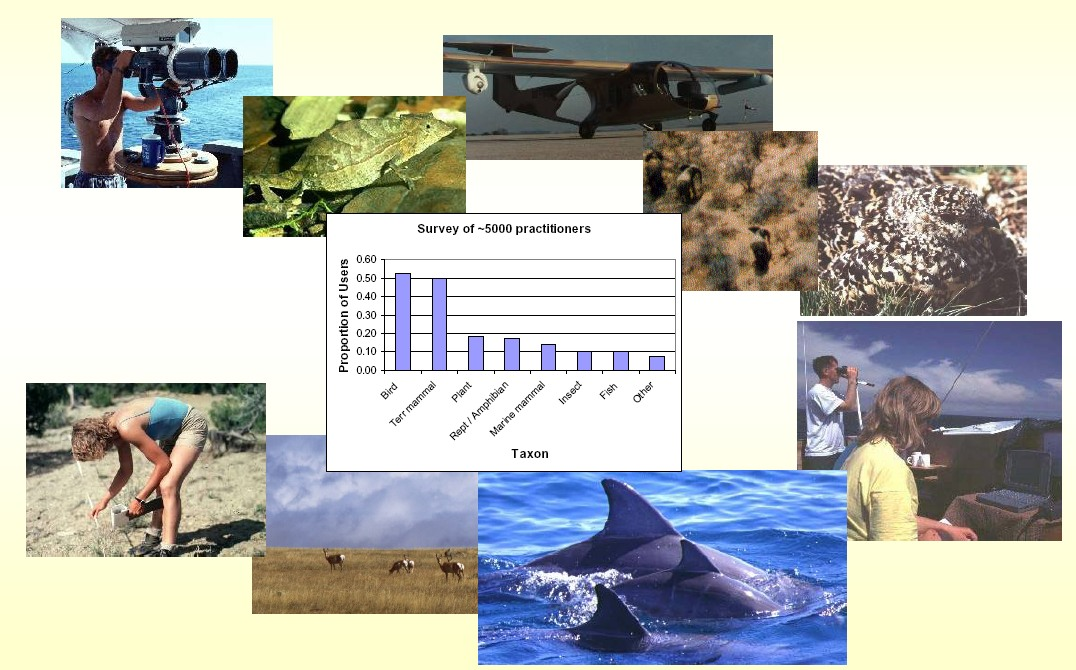
\includegraphics[height=1.9in]{ds}
    \ec}
		}
    \ei
\end{frame}

\begin{frame}[fragile]
    \frametitle{Example - distance sampling}
      \bc  
        \mode<presentation>
          {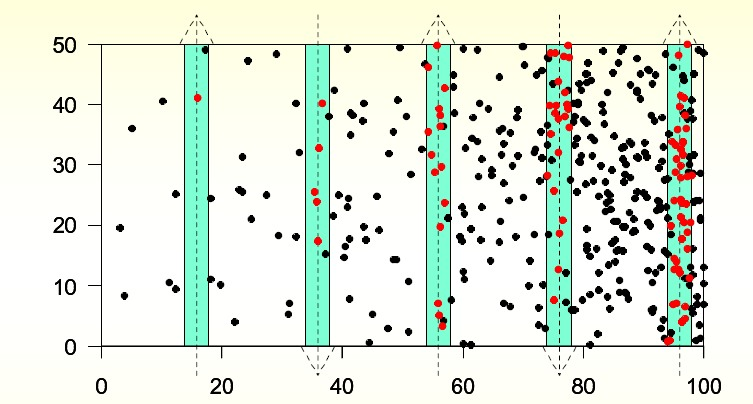
\includegraphics[height=2in]{ds2}}
         \mode<article> {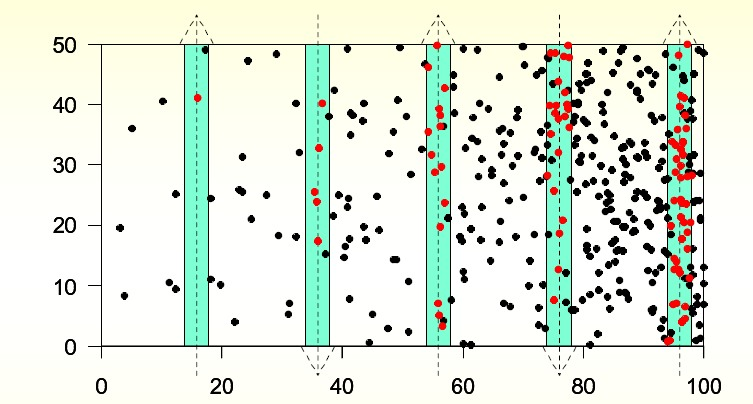
\includegraphics[height=1.5in]{ds2}}
      \ec
	\bi
	    \item Dots represent groups of animals
	    \item Red dots = detected groups; \\Black dots = undetected groups
	\ei
\end{frame}
\begin{frame}
    \frametitle{Example - distance sampling}
    \bi
        \item Density 
        \begin{eqnarray*}
        \hat{D} & =& \frac{\mbox{n seen} \times \mbox{mean group size}}
          {\mbox{area searched} \times \mbox{p detect}}\\
          & = & \frac{n \times \bar{s}}{2wL \times \hat{p}}
        \end{eqnarray*}
        %$\hat{D} = (1/2wL) n (1/\hat{p}) \bar{s}$
        \item Analytic variance $\hat{\mbox{var}}(\hat{D}) \approx \hat{D}^2
          \left( \frac{var(n)}{n^2} \times 
                 \frac{var(\bar{s})}{\bar{s}^2} \times
                 \frac{var(\hat{p})}{\hat{p}^2} \right)$
        \item Analytic CIs -- assume $\hat{D}$ lognormally distributed
        \item Alternative -- nonparametric bootstrap
        \bi
            \item Resample transects with replacement
        \ei
    \ei
\end{frame}

\subsection{Summary}

\begin{frame}
    \frametitle{Advantages}
    \bi
        \item Simple to apply
        \item General and robust (compared with other general analytic approaches) method of setting CIs
        \item No need for parametric assumption about $f()$ or quantity of interest
    \ei
\end{frame}

\begin{frame}[fragile]
    \frametitle{Disadvantages}
    \bi
      \item Assumes observations/samples are iid
	    \bi
				\item \textit{probability integral transform} method when not identically distributed)
				\item \textit{copulas} when samples are not independent
			\ei
			\item <2-> Performs poorly when underlying distribution is very skewed, or estimator is very biased.
			\bi
			  \item consider \textit{BCa (Bias corrected and accelerated) bootstrap} (see Carpinter and Bithell 2000, cited earlier).
			\ei
      \item <3-> Requires a reasonably large number of samples -- 20-30 or more\\
        (but see \textit{smoothed bootstrap}  in background reading)
      \item <4-> In complex examples, it can be difficult to see what the unit for resampling should be
      \item <5-> Generally only asymptotically exact as $b$ and $n$ $\Rightarrow \infty$
    \ei
\end{frame}

\section{Parametric bootstrap}

\subsection{How to generate resamples}

\begin{frame}
    \frametitle{Introduction}
    \bi
        \item Parametric MC method for obtaining CIs
        \item Algorithm:
            \bi
                \item Fit a parametric model $f(\theta)$ to the data
                \item Generate resamples by simulating from the fitted model
                \item Use the resamples to obtain CIs (e.g., by percentile method)
            \ei
    \ei
\end{frame}

\begin{frame}
    \frametitle{Pine martin example}
    \bi
        \item 999 resamples generated from $\mbox{N}(\bar{x},s^2)$
    \ei
\bc
        \mode<presentation>
          {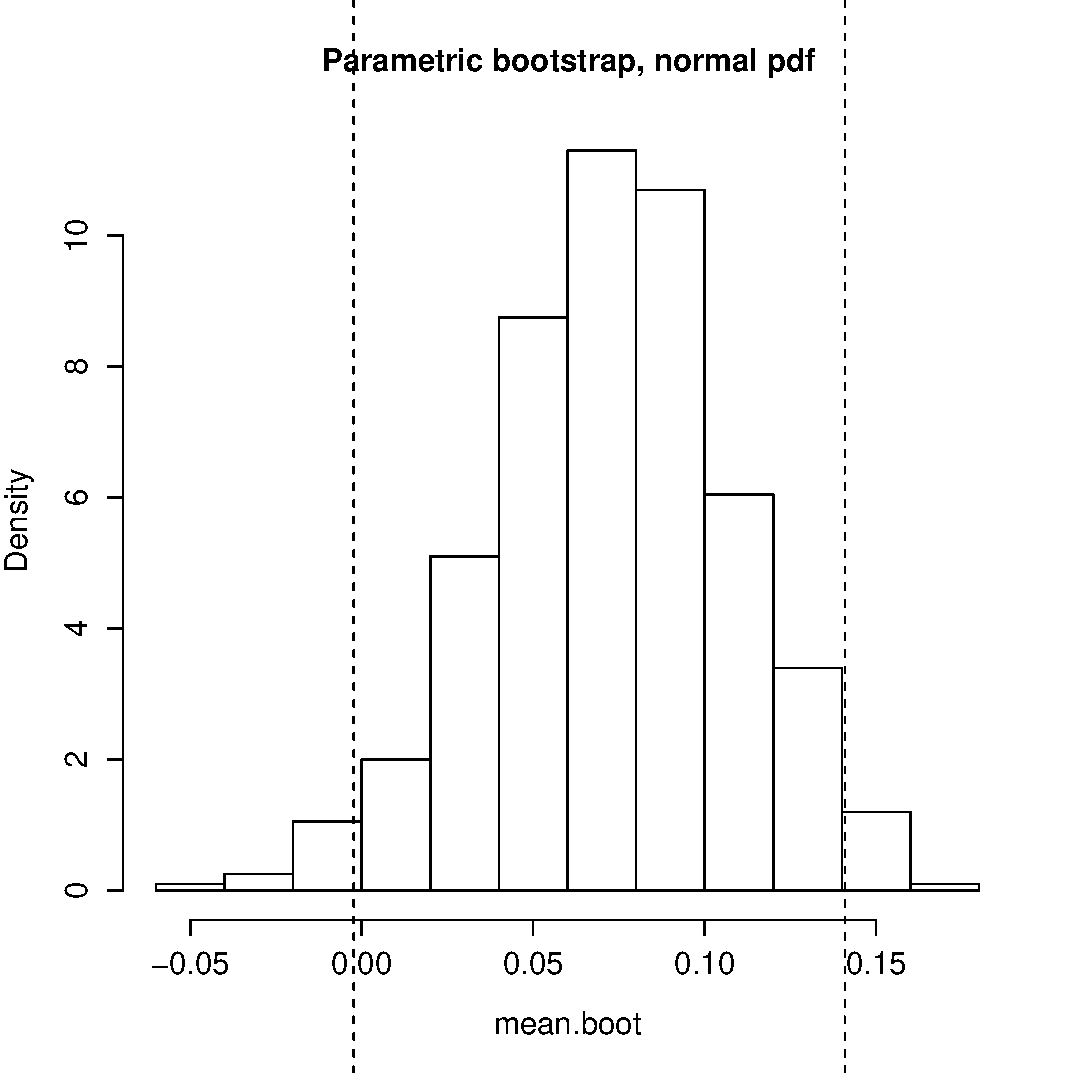
\includegraphics[height=2in]{HistMeanBootCINormal}}
        \mode<article>  {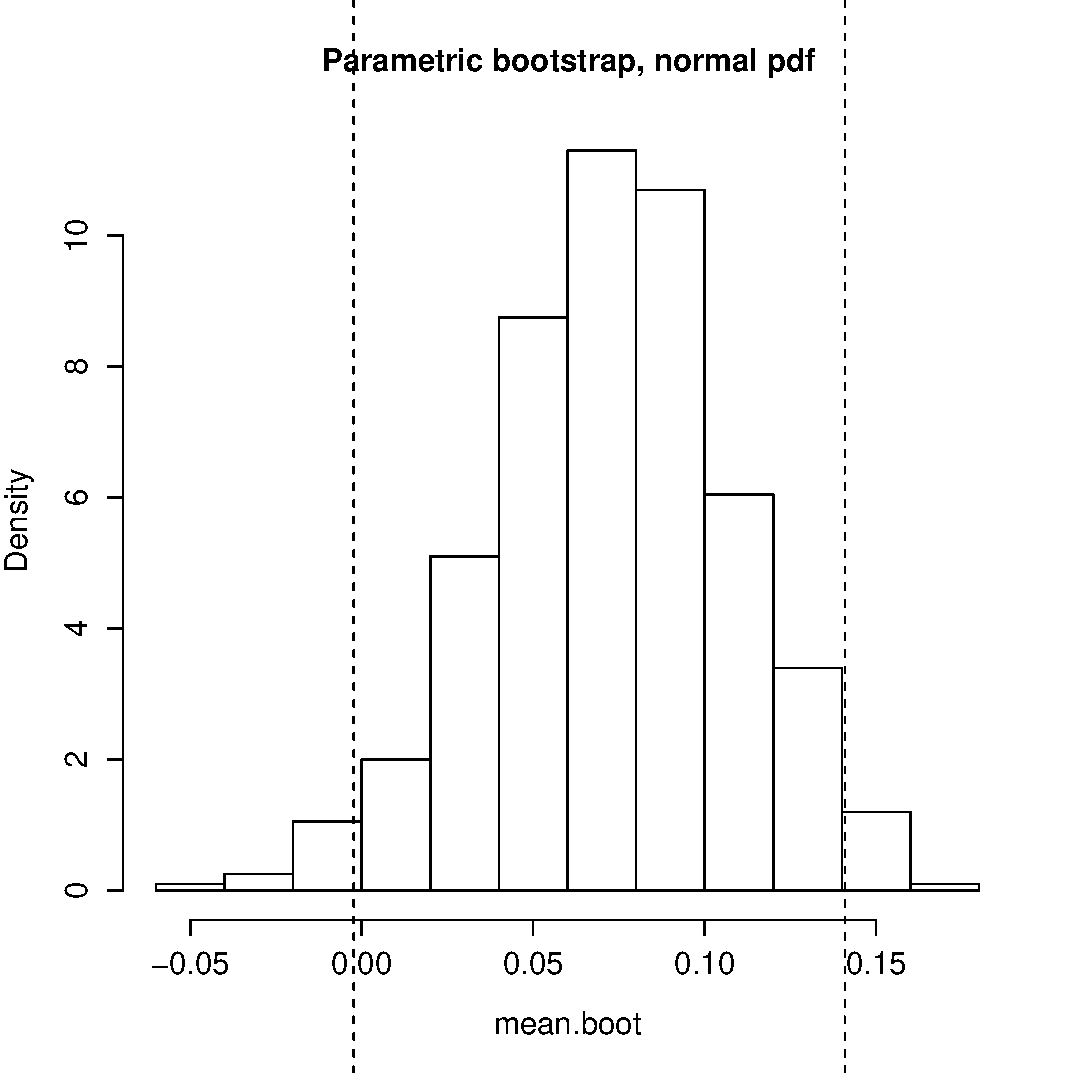
\includegraphics[height=1.5in]{HistMeanBootCINormal}}
    \ec
\end{frame}

\begin{frame}
    \frametitle{Pine martin example}
    \bi
        \item 999 resamples generated from $\mbox{t}_{11}(\bar{x},s^2)$
    \ei
\bc
        \mode<presentation>
         {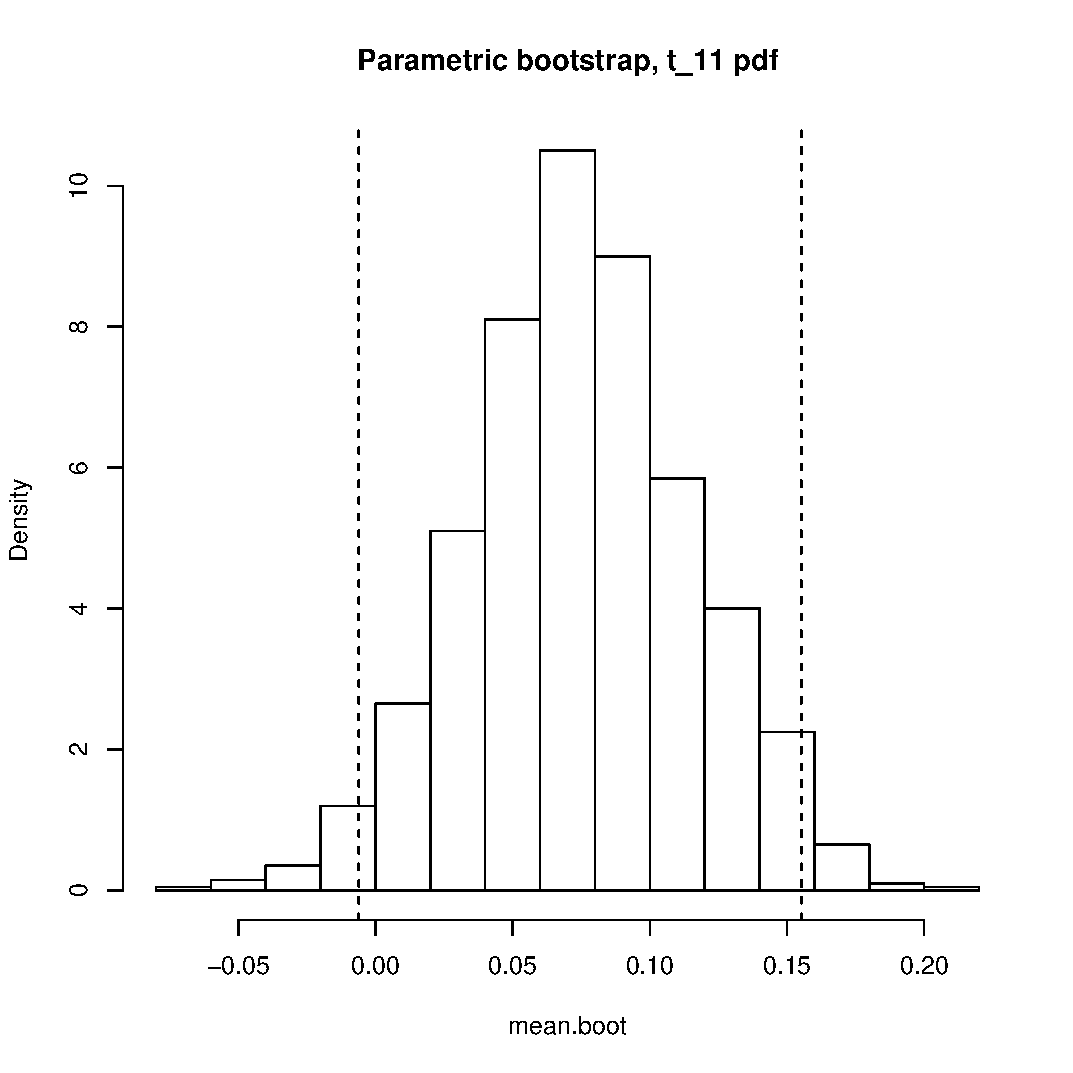
\includegraphics[height=2in]{HistMeanBootCIt}}
       \mode<article> {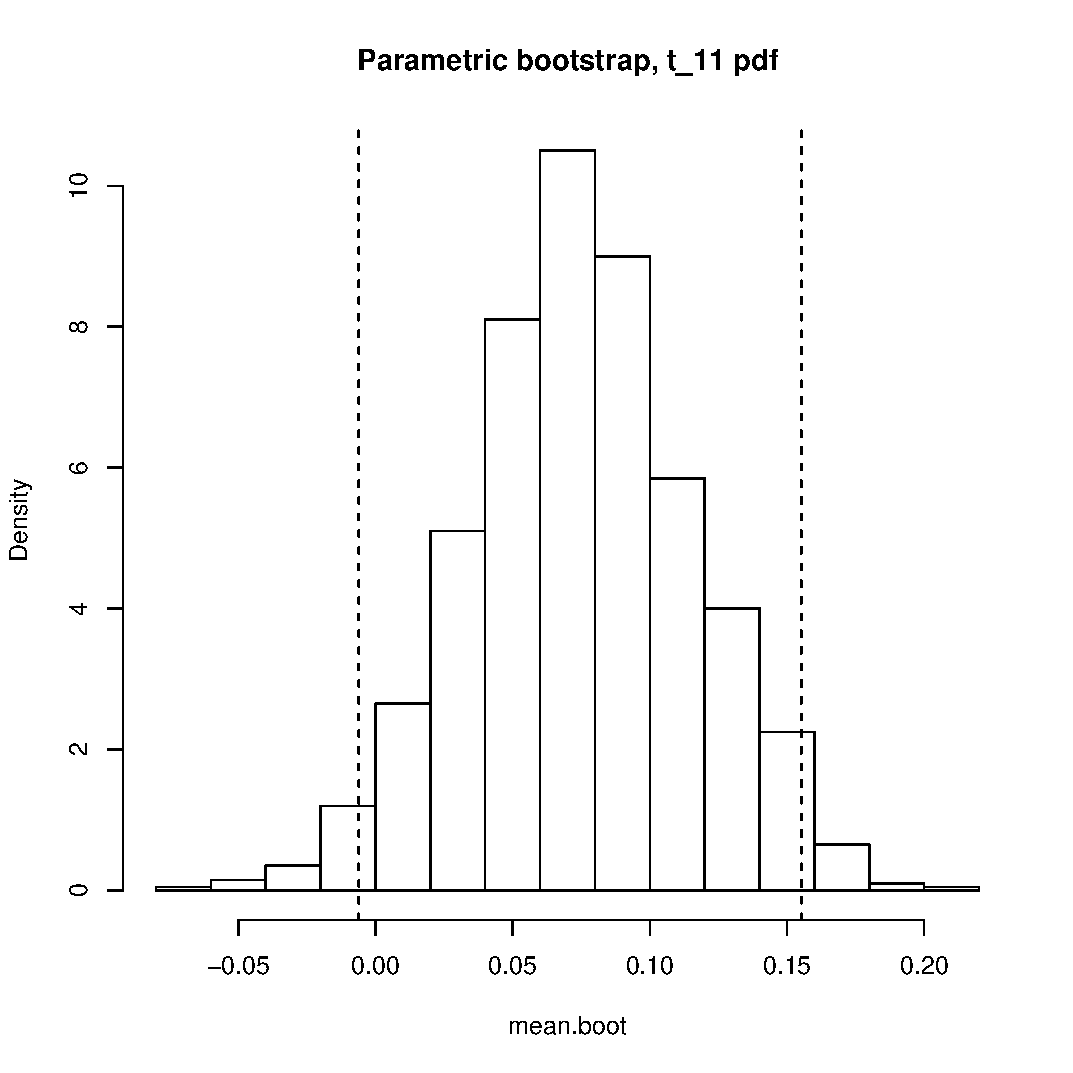
\includegraphics[height=1.5in]{HistMeanBootCIt}}
    \ec
\end{frame}

\subsection{Summary}

\begin{frame}
    \frametitle{Advantages}
    \bi
        \item General and robust (compared with general analytic approaches) method of setting CIs
        \item Observations don't need to be iid
    \ei
\end{frame}

\begin{frame}
    \frametitle{Disadvantages}
    \bi
        \item Generally only asymptotically exact as $b$ and $n$ $\Rightarrow \infty$
        \item Must assume a parametric model for $f(\theta)$
    \ei
\end{frame}

\end{document}


